\section{Analisi delle caratteristiche del dataset}
In questa fase preliminare si illustreranno le principali considerazioni fatte sul dataset fornito.
\subsection{Boxplot dei dati}
Si considerino i seguenti boxplot delle variabili del dataset.
\begin{figure}[h]
	\centering
	\subfigure[Boxplot della variabile dipendente y\_VideoQuality]{
		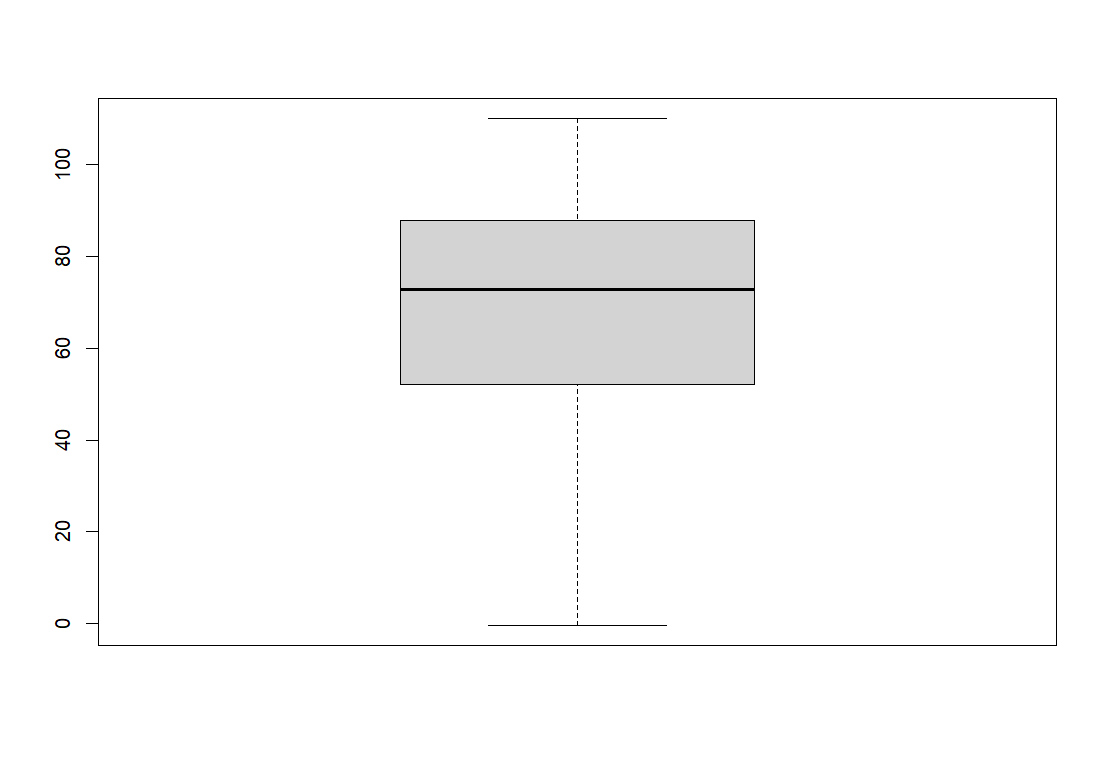
\includegraphics[width=0.65\linewidth]{../graphs/DescriptiveStatisticPlots/boxplot_y_VideoQuality}
		\label{fig:boxplotyvideoquality}
	}
	\subfigure[Boxplot delle variabili indipendenti x\_i]{
		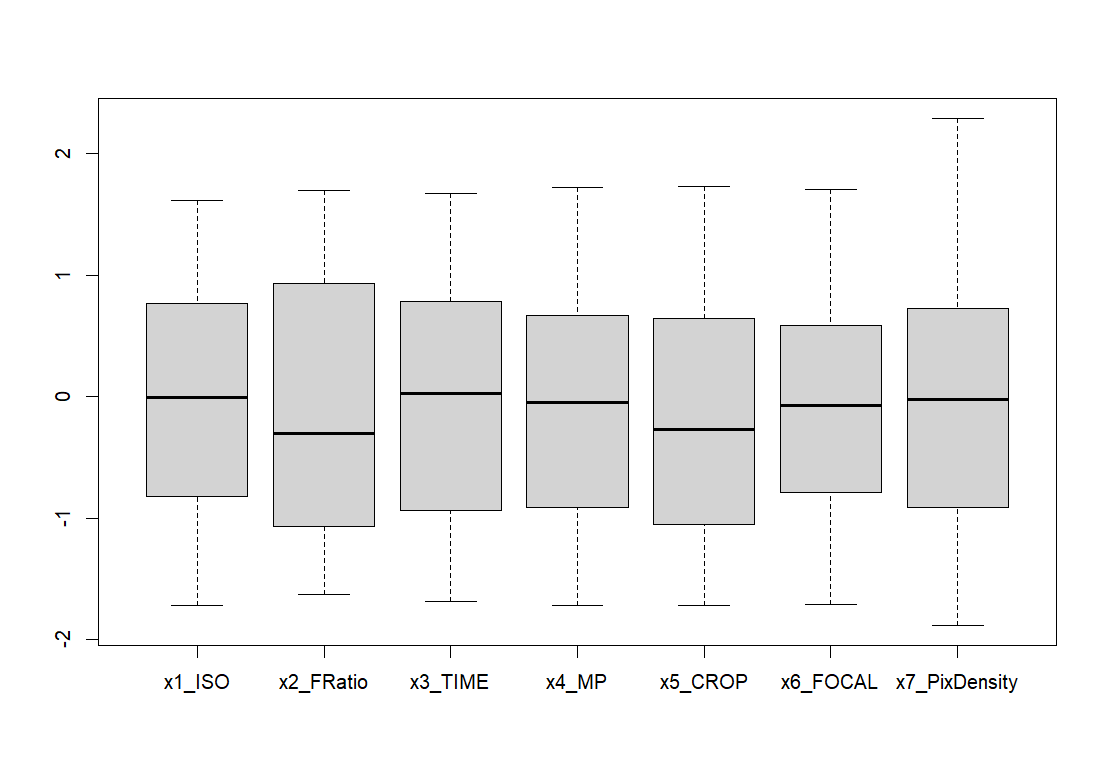
\includegraphics[width=0.65\linewidth]{../graphs/DescriptiveStatisticPlots/boxplot_all_x_i}
		\label{fig:boxplotallxi}
	}
	\caption{Boxplot delle variabili considerate}
\end{figure}

Si osservi innanzitutto che i valori per ciascuna variabile sono tutti contenuti all'interno dell'intervallo interquartile e che quindi non sono presenti outliers. Per quel che riguarda la variabile dipendente y\_VideoQuality si è osservato che il valore della media e della mediana sono simili, infatti valgono rispettivamente  $\text{media}=72.8135, \text{mediana}=68.6081$. Si è osservato inoltre che i valori assunti dalla variabile x7$\_$PixDensity coprono un intervallo maggiore rispetto alle altre variabili indipendenti. 
\subsection{Analisi di normalità}
Anche se non strettamente necessario ai fini del metodo di regressione, si è comunque deciso di verificare se qualcuna delle variabili indipendenti avesse una distribuzione normale.\begin{figure}[h]
	\centering
	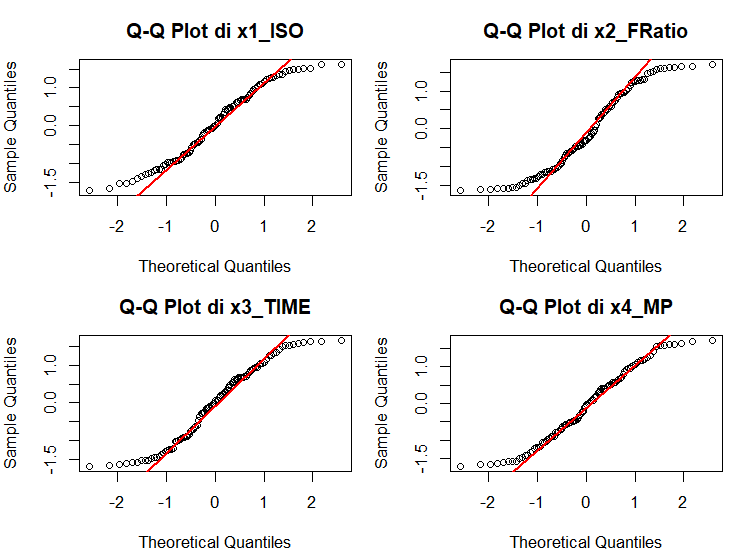
\includegraphics[width=0.9\linewidth]{../graphs/DescriptiveStatisticPlots/qqplot1/qqplot1}
	\caption{}
	\label{fig:qqplot1}
\end{figure}
Tra i diversi qq-plot, si osserva che la variabile x6$\_$Focal sembrerebbe avere una distribuzione normale. Applicando il test di shapiro a questa variabile si ottiene
\begin{align*}
	\text{W} = 0.97, \text{p-value} = 0.02.
\end{align*}
Il valore di p-value ottenuto non si discosta molto da 0.05 e si potrebbe perciò supporre che la variabile sia distribuita come una normale.
\begin{figure}[h]
	\subfigure{
		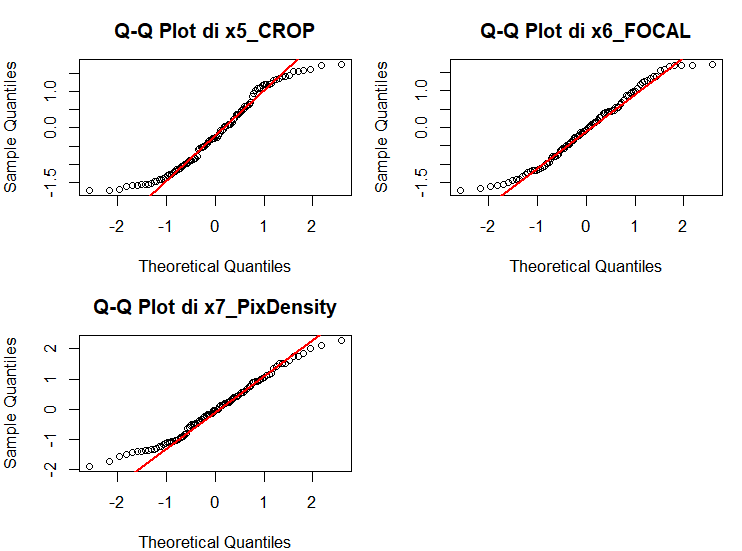
\includegraphics[width=0.9\linewidth]{../graphs/DescriptiveStatisticPlots/qqplot1/qqplot2}
		\label{fig:qqplot2}	
		}
\end{figure}




